% Paths assume the manuscript is compiled from paper/.
\begin{figure}[tbp]
    \centering
    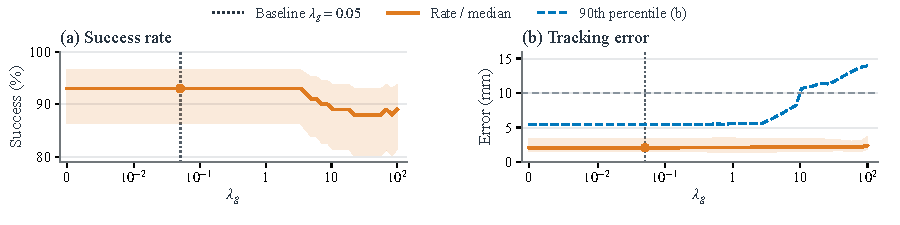
\includegraphics[width=\linewidth]{figures/reacher_lam_g_ablation/lam_g_performance.pdf}
    \caption{Regularization ablation at rank $60$ over $100$ paired development
    seeds ($211$--$310$) for each of $52$ values of $\lambda_g$.
    Panel (a) shows success rate with pointwise $95\%$ Wilson intervals.
    Panel (b) shows the median and interquartile range, including failed
    rollouts. Tracking error is each rollout's mean fingertip error over its
    last $100$ steps; the blue dashed curve is its $90$th percentile and the
    horizontal gray line marks $10$\,mm. Dotted vertical lines mark the baseline
    $\lambda_g=0.05$. The horizontal axes are logarithmic above $0.005$ and
    linear near zero.}
    \label{fig:lam-g-performance}
\end{figure}

\begin{figure}[tbp]
    \centering
    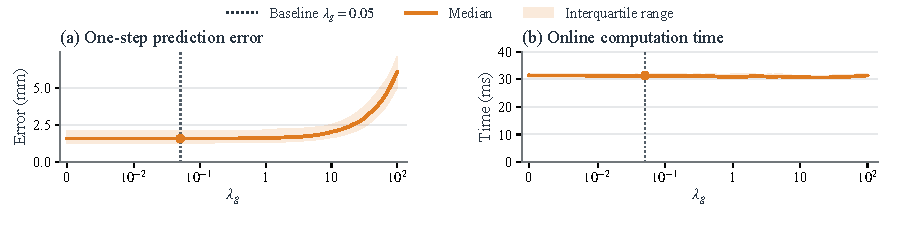
\includegraphics[width=\linewidth]{figures/reacher_lam_g_ablation/lam_g_prediction_timing.pdf}
    \caption{Prediction accuracy and online computation time for the same
    regularization sweep. Curves show medians and shaded regions show
    interquartile ranges across rollouts. Each rollout contributes its mean
    one-step fingertip prediction error in (a) and its median control-step
    time in (b), excluding the first five steps. Timings are not pooled
    per-step statistics. Runs use one worker and one numerical thread on a
    shared computer; setup, offline computation, and result writing are excluded.
    Axis conventions follow Figure~\ref{fig:lam-g-performance}.}
    \label{fig:lam-g-prediction-timing}
\end{figure}
